\documentclass[12pt,a4paper,oneside,english]{book}

\usepackage{cite}


%\usepackage[latin1]{inputenc}

%\usepackage[T1]{fontenc}
\usepackage[english]{babel}
\usepackage{amsmath}
\usepackage{amsfonts}
\usepackage{amssymb}
\usepackage{graphicx}
\usepackage{subfig}
\usepackage{fancyhdr}
\usepackage{appendix}
\usepackage{hyphenat}
\usepackage{pdfpages}
%\usepackage{tocloft} % For TOC customization ( table of contents )
\usepackage{array,multirow,makecell}
\newcolumntype{C}[1]{>{\arraybackslash}p{#1}}

\usepackage{enumitem}
\setlist{leftmargin=*,itemsep=0pt}

\usepackage{centernot}
\usepackage[linesnumbered,ruled,vlined,english,onelanguage]{algorithm2e}

\usepackage{quotchap}
\makeatletter
\renewcommand{\@makechapterhead}[1]{
 \chapterheadstartvskip
 {\size@chapter{\sectfont\raggedright
 {\chapnumfont
 \ifnum \c@secnumdepth >\m@ne
 \if@mainmatter\thechapter %frontmatter for roman numerals
 \fi\fi
 \par\nobreak}
 {\raggedright\advance\leftmargin10em\interlinepenalty\@M #1\par}}
 \nobreak\chapterheadendvskip}}
\makeatother
\renewcommand*{\chapterheadendvskip}{\vspace{2cm}}
%\renewcommand{\thechapter}{\Roman{chapter}} % Set chapter numbering to Roman numerals


\usepackage{geometry}
\geometry{hmargin=2.5cm,vmargin=2.5cm}

\pagestyle{fancyplain}
\lhead{\fancyplain{}{\nouppercase{\textit{\leftmark}}}}
\chead{\fancyplain{}{}}
\rhead{\fancyplain{}{}}
\lfoot{\fancyplain{}{}}
\cfoot{\fancyplain{}{}}
\rfoot{\fancyplain{\thepage}{\thepage}}
\renewcommand{\headrulewidth}{1pt}
\renewcommand{\footrulewidth}{1pt}

\renewcommand{\thesection}{\Roman{section}} % Set section numbering to Roman numerals % previously \arabic{section}

\usepackage{titlesec}
\titleformat{\paragraph}{\fontsize{11}{10}\bfseries}{\theparagraph}{1em}{}
\titlespacing*{\paragraph}{0pt}{10pt plus 2pt minus 0pt}{0pt plus 2pt minus 0pt}

\setcounter{secnumdepth}{4}
\setcounter{tocdepth}{4}

\usepackage{array}
\usepackage{multirow}
%\addto\captionsfrench{\def\tablename{\textsc{Tableau}}}

%\DefineBibliographyStrings{french}{urlseen = {},}

\setlength{\parskip}{8pt}
\usepackage{setspace}

\usepackage{url}

\usepackage{hyperref}
% Comment before printing to remove links' colors
\definecolor{darkblue}{rgb}{0.0, 0.0, 0.5}
\hypersetup{
 colorlinks,
 linktocpage=true,
 linkcolor={darkblue},
 citecolor={darkblue},
 urlcolor={blue}}

\sloppy

\author{You}
\title{Internship Report}

\begin{document}
\pagenumbering{gobble}
\includepdf[pages=-]{FrontPage.pdf}
\chapter*{Acknowledgments}

\frontmatter %here yothhrou les num des pages en bas 
\chapter*{Abstract}
\normalsize{Write your abstract here.

\medskip
{\noindent \textbf{Keywords: ..., ... .} }

\spacing{1}
\tableofcontents{}
\newpage 
\listoffigures
\newpage 
\listoftables
\newpage
\spacing{1.4}
\chapter*{List of acronyms}
%\addcontentsline{toc}{chapter}{Liste des acronymes}
\markboth{List of acronyms}{}
\begin{itemize}
\item \textbf{Abbrev.} Abbreviation
\end{itemize}

\frontmatter %here yothhrou les num des pages fl contnent
%\frontmatter  %to have roman page numbering in the beginning
%\mtcaddchapter[Introduction g�n�rale]


\chapter*{Introduction}
\addcontentsline{toc}{chapter}{Introduction}
\markboth{Introduction}{}


\chapter{Company Presentation}
\label{ch:1er}
\section{Overview}
Founded in 2020, and located in both Meudon la forêt , Meudonn France and tunis, Tunisia, 
Hydatis is dedicated to helping early-stage companies leverage the latest data intelligence and digital technologies to solve real-world challenges, becoming, since then, a leading technology startup studio with a proven track record.
\begin{figure}[h!] % placement options: h=here, t=top, b=bottom, p=page
    \centering
    
\includegraphics[width=0.2\textwidth]{images/hydatiss.png}
    \caption{Logo of Hydatis}
    \label{fig:hydatis}
\end{figure}

Hydatis specializes in AI, machine learning, blockchain, big data Analysis and more. Hydatis's team of technology experts is dedicated to building scalable and sustainable businesses, with a focus on creativity, strategy, and technology alongside with a vast network of partners and investors and a strong reputation in the technology industry.
\begin{figure}[h!] % placement options: h=here, t=top, b=bottom, p=page
    \centering
    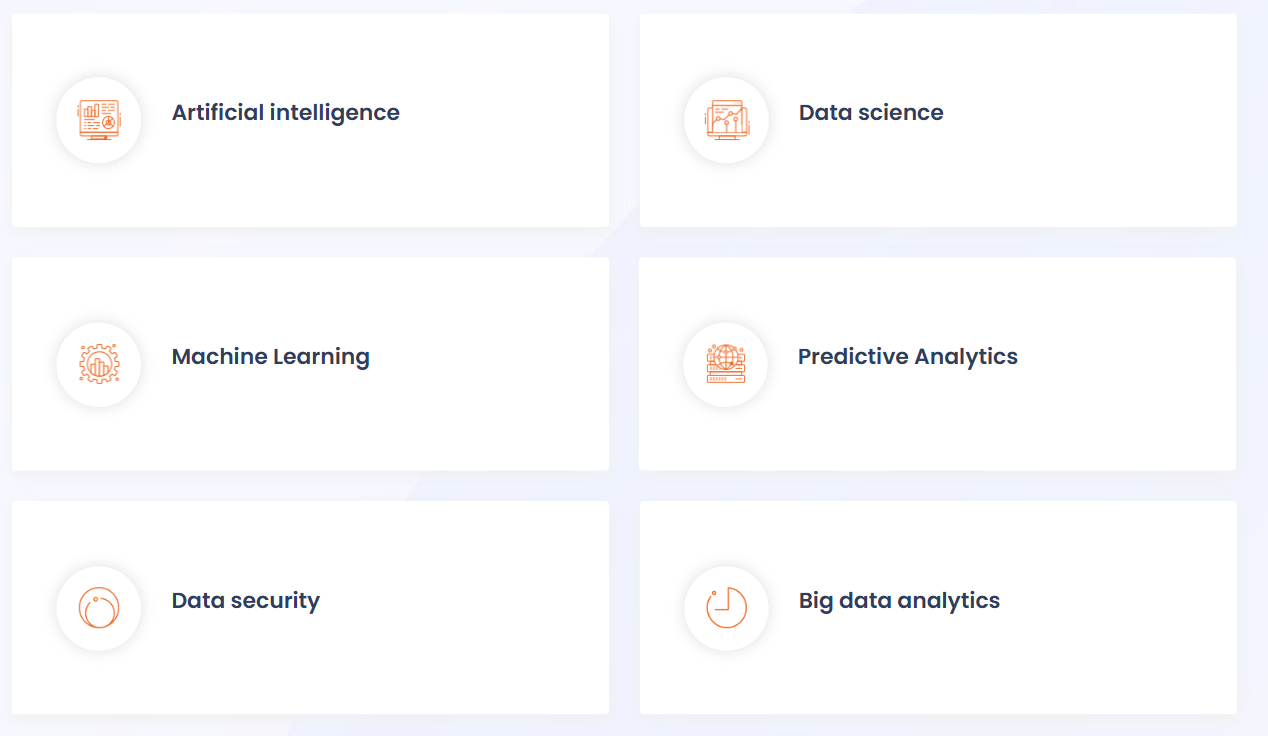
\includegraphics[width=0.699\textwidth]{images/Expertise_hydatis.png}
    \caption{Hydatis' Areas of Expertise}
    \label{fig:Expertise_hydatis}
\end{figure}

\section{Sectors of Activities}%and services offered
Hydatis is a product-focused Tech venture studio offering a range of services tailored to the unique needs of each startup, including:
 business planning, product development, marketing, and fundraising. 
%With their expertise in data analytics, machine learning, and other advanced technologies, 
Leveraging technology and entrepreneurship, they help clients turn data into actionable insights that drive business success.
%help businesses make big decisions about their future by making tangible versions of tomorrow.
\subsection{Services offered}
\begin{itemize}
    \item \textbf {Software development Services}
    \item \textbf{CTO as a service}
    \item \textbf{IT Consulting}
    \item \textbf{Devops Consulting}
    \item \textbf{and a lot more...}
\end{itemize}
\begin{figure}[h!]
    \centering
    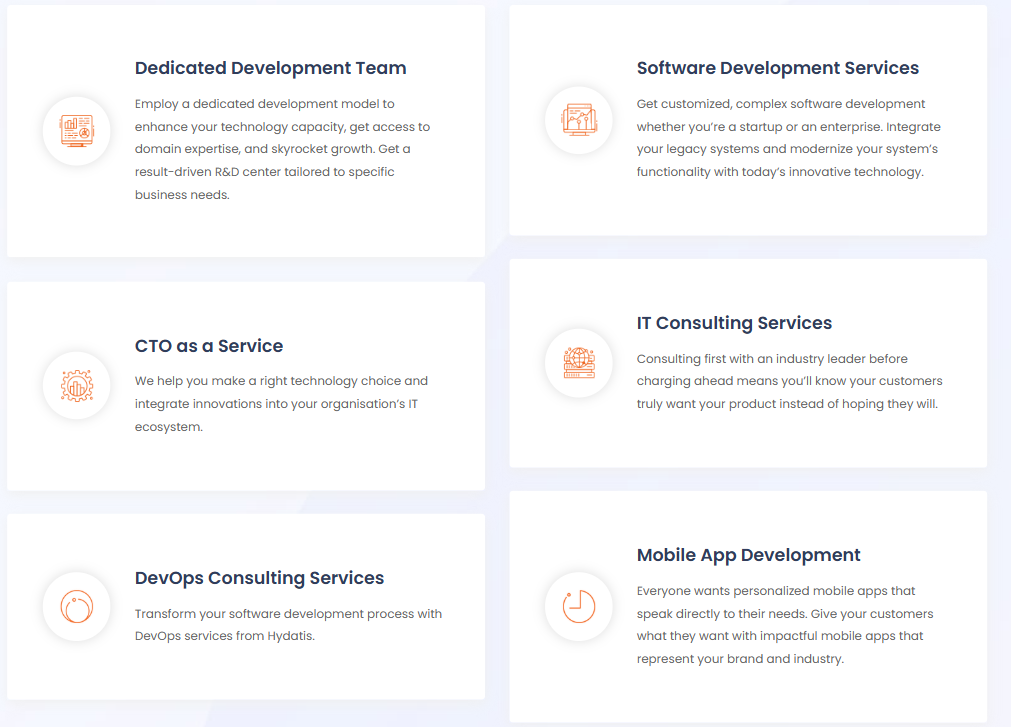
\includegraphics[width=0.9\textwidth]{images/services_hydatis.png}
    \caption{Hydatis' Services}
    \label{fig:Services_hydatis}
\end{figure}

\section{Organizational structure and Human Capital}

\chapter{Theoritical Foundations and State of the Art}
\label{ch:2eme}
\section{Geospatical Analysis for Risk Prediction}
\subsection{Anomaly Detection in Geographical Information Systems}
%create abstract GIS 
%the subsections will be discussed later
\section { Vocal Signal Processing for Distress Detection}
\section{Machine Learning for Behavioral Anomaly Detection}


\chapter{Design and implementation}
\label{ch:3eme}
\section{System Architecture and Data management}
\section{Implementation of the Geospatial Analysis Module}
\section{Implementation of the Vocal Signal Processing Pipeline}
\section{Implementation of the Behavioral Profiling Module} % or the Behavioral Anomaly Detection Module or the Machine Learning Module
\section{Final Decision Engine and System Integration}
%this may be merged with the first section (dont know shkoun shyemshi bahtha sahbou ( hawka naamlou referencing lel sections elli will tailor the details if nkaddmou el decision engine kbal les ai modules))

\chapter{Results and Discussion}

\section{Evaluation and Results}
\section{Discussion}








%\section*{Conclusion}
%\section{Conclusion}
\chapter*{Conclusion and perspectives}
\addcontentsline{toc}{chapter}{Conclusion and perspectives}
\markboth{Conclusion and perspectives}{}

\begin{appendix}
\chapter{Appendix 1}
Insert your appendixes here if you need.
\end{appendix}

%\spacing{1}
\bibliographystyle{unsrt}
\bibliography{references}
\end{document}